\documentclass[11pt]{article}
\usepackage{fullpage}
\usepackage{graphicx}
\usepackage{natbib}

\begin{document}
\title{Radio Skillz: Analog Lab 2}

\maketitle

\section*{Prerequisites}

Reading: Horowitz \& Hill, Ch. 2

\begin{itemize}
\item Transmission Lines
\item Transistors
\item Amplifier Circuits
\end{itemize}

\section*{Materials}

\begin{itemize}
\item rope and string of various thicknesses (pretty long)
\item breadboard
\item misc R, C, transistor components
\item power supply
\item function generator w/ external FM reference
\item oscilloscope w/ probes
\item voltimeter
\item speaker w/o amplifier
\item long cable (as long as possible, longer than 100m would be great)
\end{itemize}

\section*{Some Thoughts}

\subsection*{Transistors}

\begin{figure}\centering
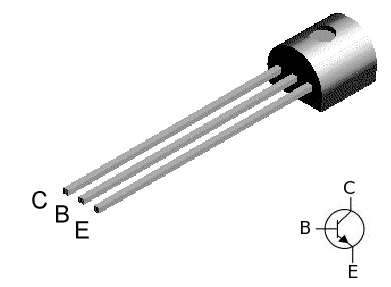
\includegraphics[width=2in]{analog_lab_2_plots/npn_transistor_pins.png}
\caption{Pinout for a generic NPN transistor (e.g. 2N3904)}
\label{fig:npn_transistor_pins}
\end{figure}

We'll be using an NPN bipolar junction transistor in this lab (see Figure \ref{fig:npn_transistor_pins}).  With
the flat face to you, pins typically read, from left to right, emitter, base, collector.  Now you know.

\subsection*{Speakers}

Last week, we just stuck our signal into an amplifying speaker and didn't think much about it.  This weak, since we are building our own amplifier, you might be wondering what's left that makes a ``speaker.''  Speakers aren't
that complicated.  At their simplest, they are solenoids that push/pull on a small magnet
attached to a diaphram.  Depending on which direction current is made to flow through the solenoid by an
alternating voltage signal, a magnetic field is set up that attracts or repels the magnet on the diaphram.  The
diaphram translates the resulting motion into pressure waves that propagate through the air.

\subsection*{Termination}

At the end of this lab, we'll be playing with some 50$\Omega$ (and maybe some 75$\Omega$) cable, examining how
waves are reflected and transmitted.  Of course, now you also have a better idea of why the oscilloscope
has selectable termination, and why it might be different depending on whether you connect as scope probe
or a BNC cable to the input.  Now that you know why and how, you have no excuse not to exercise good termination
practices!

\section{Impedance Mismatches on Rope}

\begin{itemize}
\begin{figure}[h]
\centering
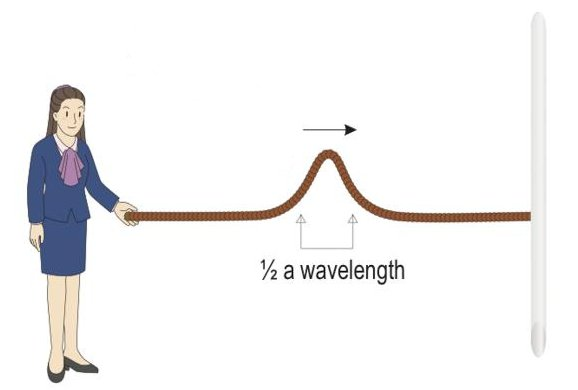
\includegraphics[width=2in]{analog_lab_2_plots/rope_pulse.jpg}
\caption{Sending a pulse down a rope}
\end{figure}
\item Get several lengths of ropes of different thicknesses.  Tie them together and tie the end of the thinner
rope to a doorknob or some other stable structure.  Hold the untied end, pull the rope relatively taut, and
then, with a quick up-down movement of the hand, send a pulse down the rope.  Observe what happens at
the interface between the ropes, and at the doorknob.
\item Switch the rope around so that the thicker end is now tied to the doorknob.  Repeat the above.  Any
difference?  
\item What would happen, do you think, if the far end of the rope, instead of being tied to a fixed point,
was tied to a ring that could move up and down on a pole?
\item Any idea how to stop the wave from reflecting off the far end of the rope?
\item If you have two thick ropes joined by a very short thin piece (small with respect to the
wavelength of the signal), what happens at that interface?
\item What about vice versa (thin ropes joined by a short thick piece)?
\end{itemize}

\section{Impedance Mismatches in a Transmission Line}

\begin{itemize}
\item Get a function generator that can output square waves.
Get a long stretch of cable and connect the function generator output to one
end of the cable.  Leave a point that you can probe with an oscilloscope.
\item Use an oscilloscope to try to detect the reflected wave.  Draw the superposition of 
transmitting and reflecting waveforms that produces your output.
\item How long is your cable?  How fast did your
pulse travel?  (BTW, it can be helpful to know that, round-about, light travels 1 ft in 1 ns, and that
waves on a cable can be up to a factor of 2 slower than that.)
\item Use a 10$\Omega$ resistor to terminate the far end of the cable.  Observe the change.
\item Now properly terminate the far end, and recover your waveform!  What was the impedance of the cable?
\end{itemize}

\section{Building an Follower}

\begin{figure}[h!]\centering
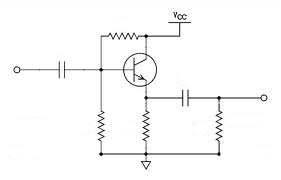
\includegraphics[width=3in]{analog_lab_2_plots/biased_emitter_follower.png}
\caption{An emitter follower that uses a biasing circuit.}
\label{fig:emitter_follower}
\end{figure}

\begin{itemize}
\item Build the emitter-follower circuit shown in Figure \ref{fig:emitter_follower}, choosing approprite
values for resistors and capacitors.  Use a 2N3904 transistor, or a similar substitute NPN BJT.  You will
power the circuit with $V_{cc}=+5V$, and will want to amplify signals in the range 100Hz to 50kHz.  Mind
your R's and C's!
\item Measure the bias voltage $V_{BE}$.
\item What is the purpose of the emitter resistor (that is, the resistor most immediately connected to the
emitter)?
\item Input a 10 kHz sine wave with 1V amplitude.  What is the relationship between the input and output voltages?
\item Predict first, and then measure, the maximum sine amplitude for which this circuit correctly operates.
\item Measure the bias voltage at the base.  How small can you make the emitter resistor before it changes?  You
might need to make the resistors in your bias circuit large so that you don't burn up the emitter resistor.
\end{itemize}

\section{Building an Amplifier for our FM radio}

\begin{figure}[h!]\centering
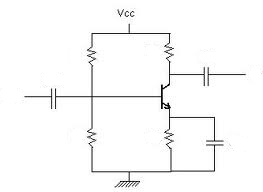
\includegraphics[width=3in]{analog_lab_2_plots/bjt_amplifier_lab2.png}
\caption{An amplifier based on an NPN BJT.}
\label{fig:amplifier}
\end{figure}

\begin{itemize}
\item Build the amplifier circuit shown in Figure \ref{fig:amplifier}, choosing appropriate values for
resistors and capacitors, using the same constraints as for the follower circuit above, and choosing a
DC gain of 2.  For the time being, omit the emitter capacitor.
\item What is the voltage at the collector?
\item Input a 10 kHz sine wave with 100mV amplitude.  What is the relationship between the 
input and output voltages?  If you did not achieve a gain of 2, why not?
\item Predict first, and then measure, the maximum sine amplitude for which this circuit correctly operates.
\item Now add in the emitter capacitor to select for a gain of 10 at 10kHz.  Again, mind your R's and C's!
\item Input a 10 kHz sine wave with 100mV amplitude.  What is the relationship between the 
input and output voltages?  If you did not achieve a gain of 10, why not?
\item Predict first, and then measure, the gain at 20 kHz.
\item Can you think of a way to make this circuit have the same gain across our whole band of interest?
\item Finally, attach a passive speaker to the output, your passive FM demodulator to the input, and bask in
the sound of your success.  You'll need to pay attention to the impedance of the speaker, and plan accordingly.
\end{itemize}

\end{document}
